%================================================================
%\chapter{Analysis of the Hodgkin-Huxley Model}
\chapter{Analysis of the Neuroscientific Models}
%================================================================

%================================================================
\section{The Hodgkin-Huxley Model}
%================================================================

\subsection{Observed data}

Observed data 

\begin{figure}[H]
    \centering
    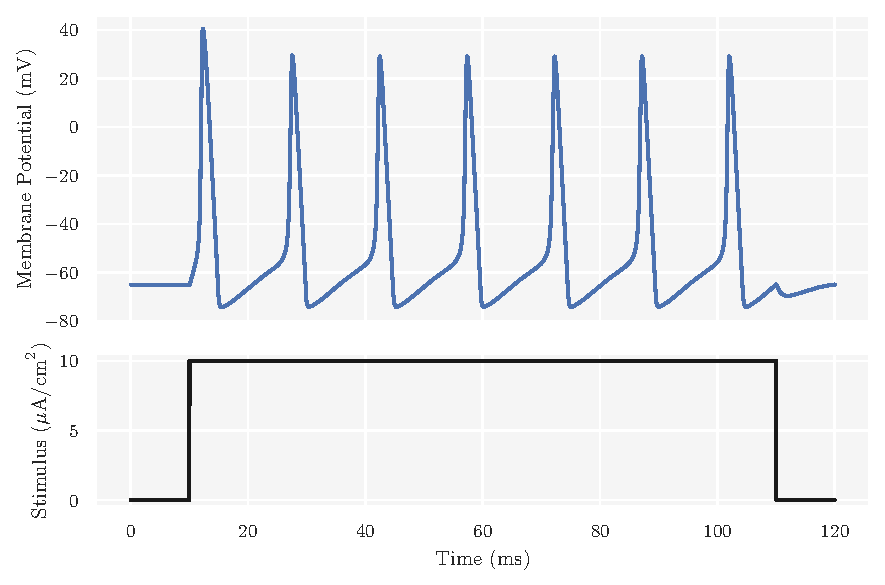
\includegraphics[scale=0.9]{hh_obs_data}
    \caption{caption}
    \label{fig:fig1}
\end{figure} 

Found locations in voltage trace for extraction of summary statistics 

\begin{figure}[H]
    \centering
    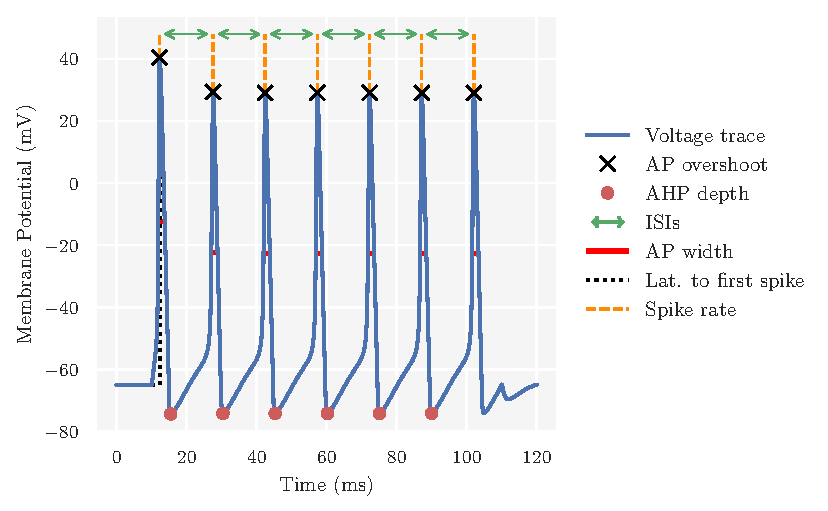
\includegraphics[scale=1]{hh_stat_extraction}
    \caption{caption}
    \label{fig:fig1}
\end{figure} 

table of observed summary statistics 

% Alternating row colors
\begin{table}[H]
  \caption{Generic table with alternating rows and different sized rulers. The number of spikes is not used as a summary statistic in and of itself, but is included to show that the statistic extraction indeed finds all spikes.}
  %\footnotesize%
  \begin{center}
    \rowcolors{2}{gray!15}{white}
    \begin{tabular}{cccc}
      \toprule
      \textbf{Summary statistic} & \textbf{Observed value} \\
      \midrule
      Number of spikes &  7 \\
      Spike rate &  0.0700 mHz \\
      Average AP overshoot & 30.7316 mV  \\
      Average AP width &  2.0501 mV \\
      Average AHP depth & -74.2234 mV \\
      Latency to first spike & 2.3000 ms \\
      Accommodation index &  $2 \cdot 10^{-17}$ \\
      \bottomrule
    \end{tabular}
  \end{center}
  \label{tab:hh_obs_sumstats}
\end{table}


\subsection{A deeper look into the statistics}

Priors for HH

\begin{figure}[H]
    \centering
    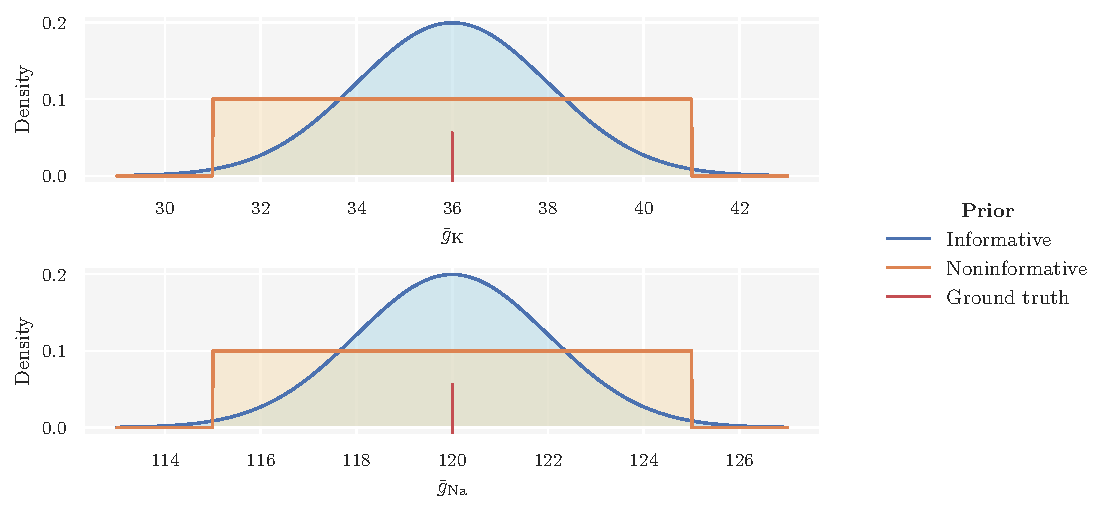
\includegraphics[scale=0.8]{hh_priors}
    \caption{caption}
    \label{fig:fig1}
\end{figure} 


Summary statistics under the (informative) prior predictive distribution (draw 2000 samples, dropna -> left with 1881 samples, but here we only plot a subset of 470 samples)

\begin{figure}[H]
    \centering
    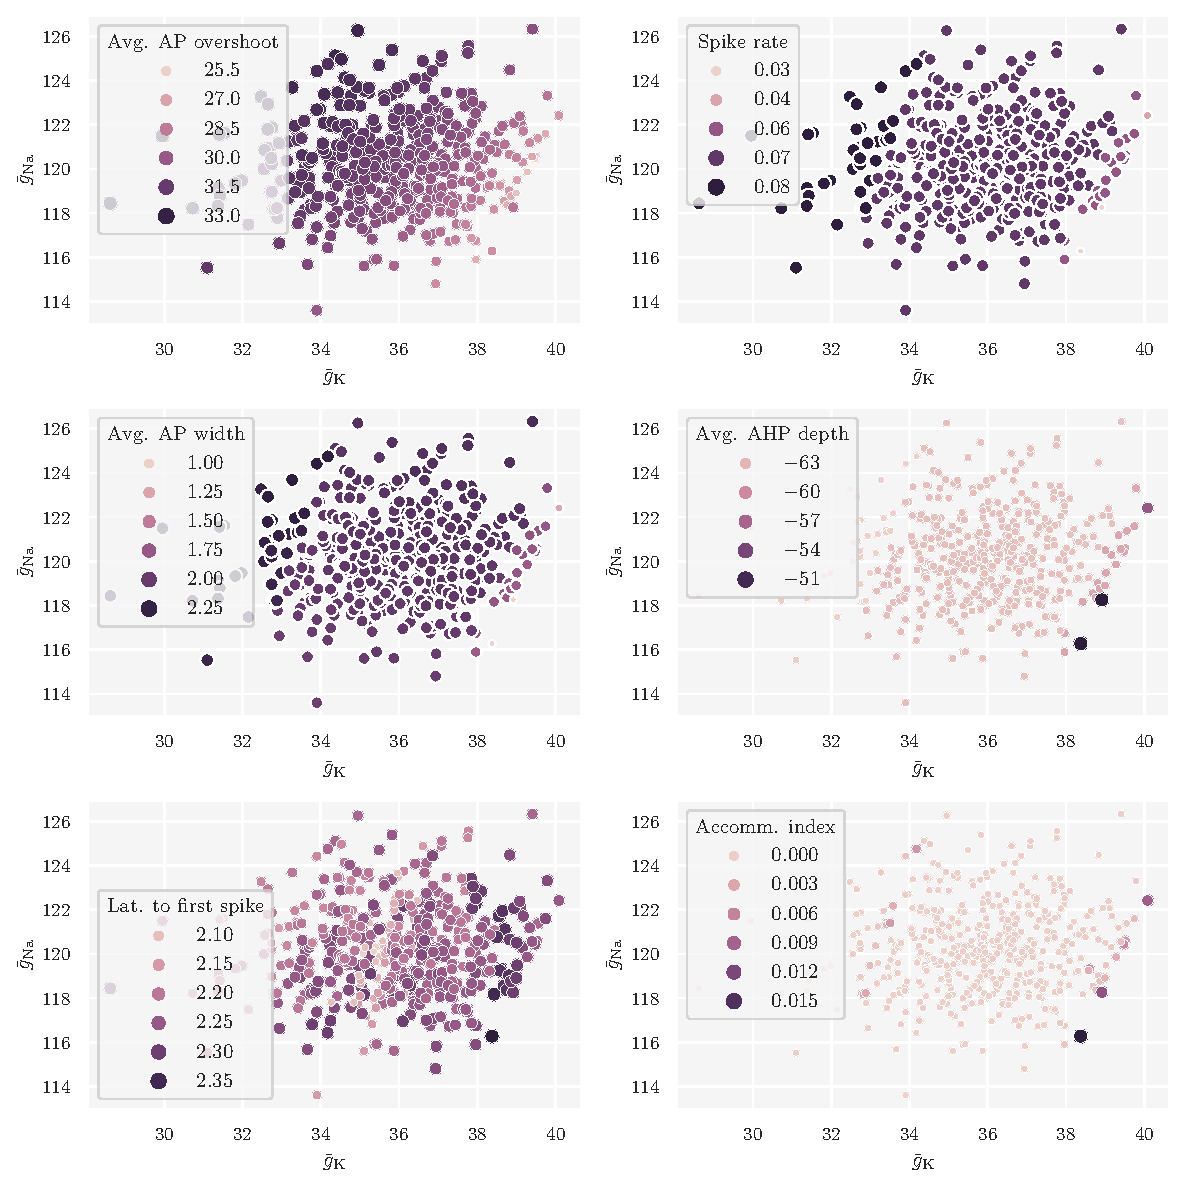
\includegraphics[scale=0.8]{hh_priorpred_sstats_normal}
    \caption{caption}
    \label{fig:fig1}
\end{figure} 


Correlation (pearson) 

\begin{figure}[H]
    \centering
    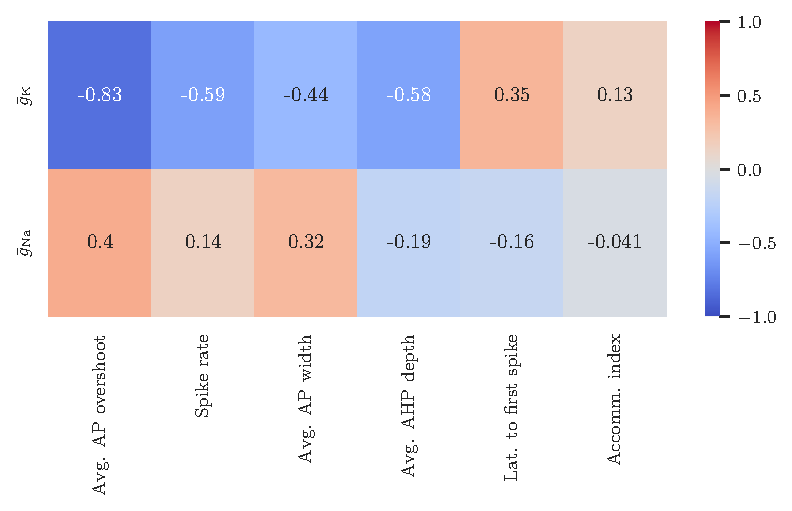
\includegraphics[scale=0.8]{hh_priorpred_corr_normal}
    \caption{caption}
    \label{fig:fig1}
\end{figure} 

weights from corr coef

\begin{figure}[H]
    \centering
    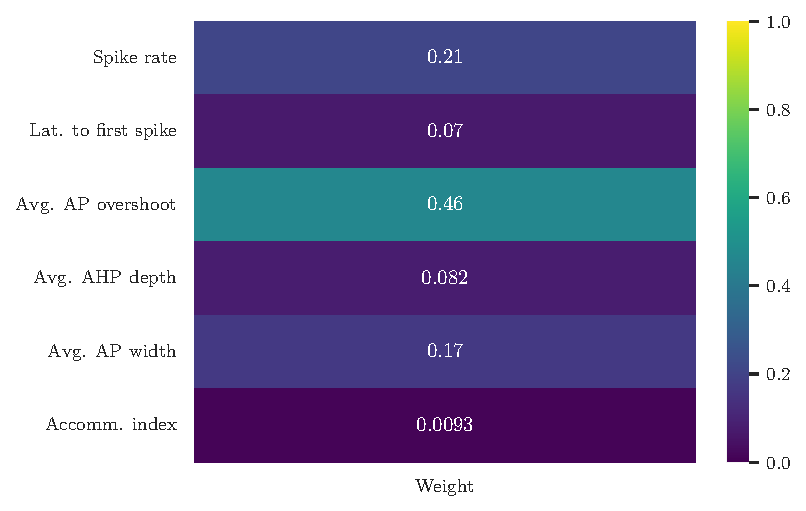
\includegraphics[scale=0.8]{hh_priorpred_weights_normal}
    \caption{caption}
    \label{fig:fig1}
\end{figure} 

Perhaps unsurprisingly, since the prior distribution does not alter the inherent relationship between the quantities, we obtain the same weights from the summary statistics generated under the noninformative prior predictive distribution. The same results as above for the noninformative prior can be found in ... ref appendix A section ...

%


\subsection{Noisy HH Data}

\begin{figure}[H]
    \centering
    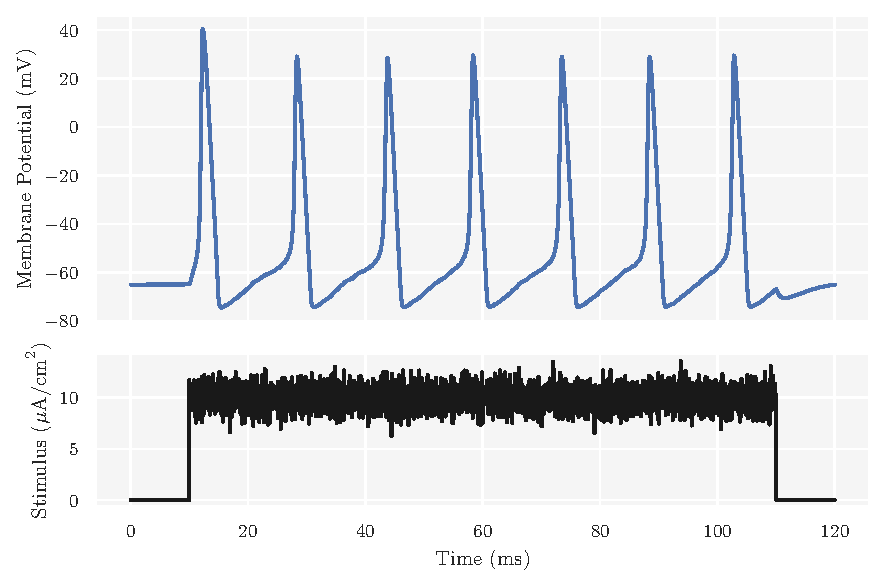
\includegraphics[scale=0.9]{hh_noisy_data}
    \caption{caption}
    \label{fig:fig1}
\end{figure} 


% Alternating row colors
\begin{table}[H]
  \caption{Generic table with alternating rows and different sized rulers. The number of spikes is not used as a summary statistic in and of itself, but is included to show that the statistic extraction indeed finds all spikes.}
  %\footnotesize%
  \begin{center}
    \rowcolors{2}{gray!15}{white}
    \begin{tabular}{cccc}
      \toprule
      \textbf{Summary statistic} & \textbf{Observed value} \\
      \midrule
      Number of spikes &  7 \\
      Spike rate &  0.0700 mHz \\
      Average AP overshoot & 30.7223 mV  \\
      Average AP width & 2.0679 mV \\
      Average AHP depth & -74.3394 mV \\
      Latency to first spike & 2.2750 ms \\
      Accommodation index &  -0.0067 \\
      \bottomrule
    \end{tabular}
  \end{center}
  \label{tab:hh_noisy_sumstats}
\end{table}



----

observed data w/o noise 

feature extraction 

plot features 

compute weights (plot correlation matrix) 

plot priors (informative, noninformative)


---

create the observed data

summary statistics of observation 

summary statistics from prior predictive

weights

(observed data with noise; same as above)

%================================================================
\section{The Brunel Network Model}
%================================================================

create the observed data

summary statistics of observation 

summary statistics from prior predictive

weights


%================================================================
\chapter{Parameter Identification with REJ-ABC}
%================================================================

%================================================================
\section{Rejection ABC Posteriors on Conductance Parameters}
%================================================================

show how Hodgkin–Huxley model is more tightly constrained by increasing numbers of data features

We also inferred HH parameters for 8 in vitro recordings from the Allen Cell Types database using the same current-clamp stimulation protocol as in our model [60, 70] (Fig. 4F, Supplementary Fig. 8). In each case, simulations based on the SNPE-inferred posterior closely resembled the original data (Fig. 4F). We note that while inferred parameters differed across recordings, some parameters (the spike threshold, the density of sodium channels, the membrane reversal potential and the density of potassium channels) were consistently more strongly constrained than others (the intrinsic neural noise, the adaptation time constant, the density of slow voltage-dependent channels and the leak conductance) (Supplementary Fig. 8). Overall, these results suggest that the electrophysiological responses measured by this current-clamp protocol can be approximated by a single-compartment HH model, and that SNPE can identify the admissible parameters.

%================================================================
\subsection{ABC Settings for Identification of Hodgkin-Huxley Parameters}
%================================================================

RMSE averaged over 10 posteriors for each quantile value. 1000 posterior samples in each posterior. 

\begin{figure}[H]
    \centering
    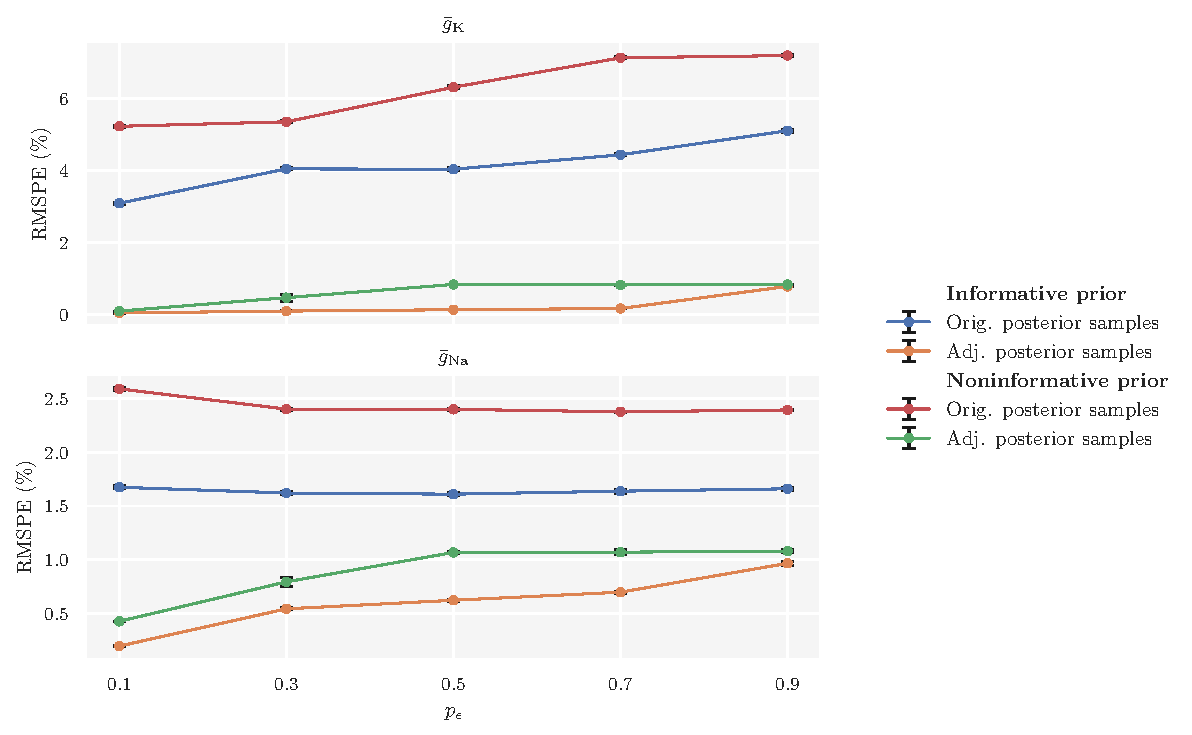
\includegraphics[scale=0.8]{RMSPE_vs_quantile}
    \caption{caption}
    \label{fig:fig1}
\end{figure} 

Run time

\begin{figure}[H]
    \centering
    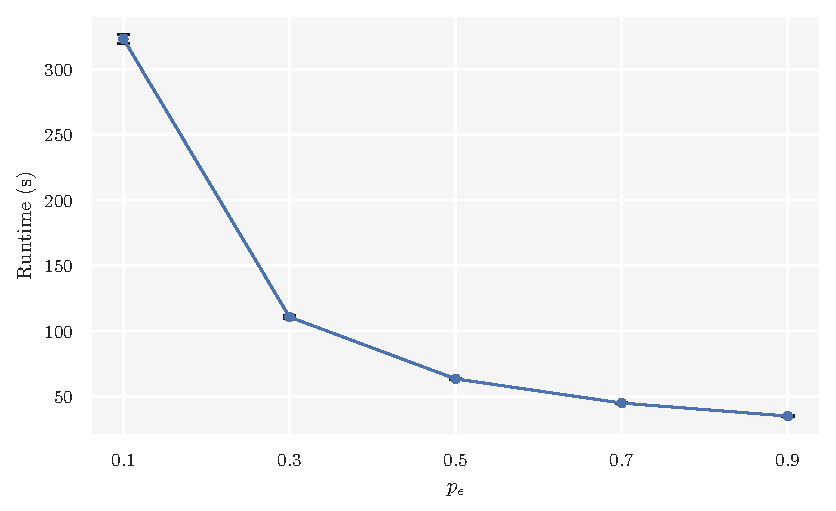
\includegraphics[scale=0.8]{comp_time_quantile}
    \caption{caption}
    \label{fig:fig1}
\end{figure}


Number of summary statistics

\begin{figure}[H]
    \centering
    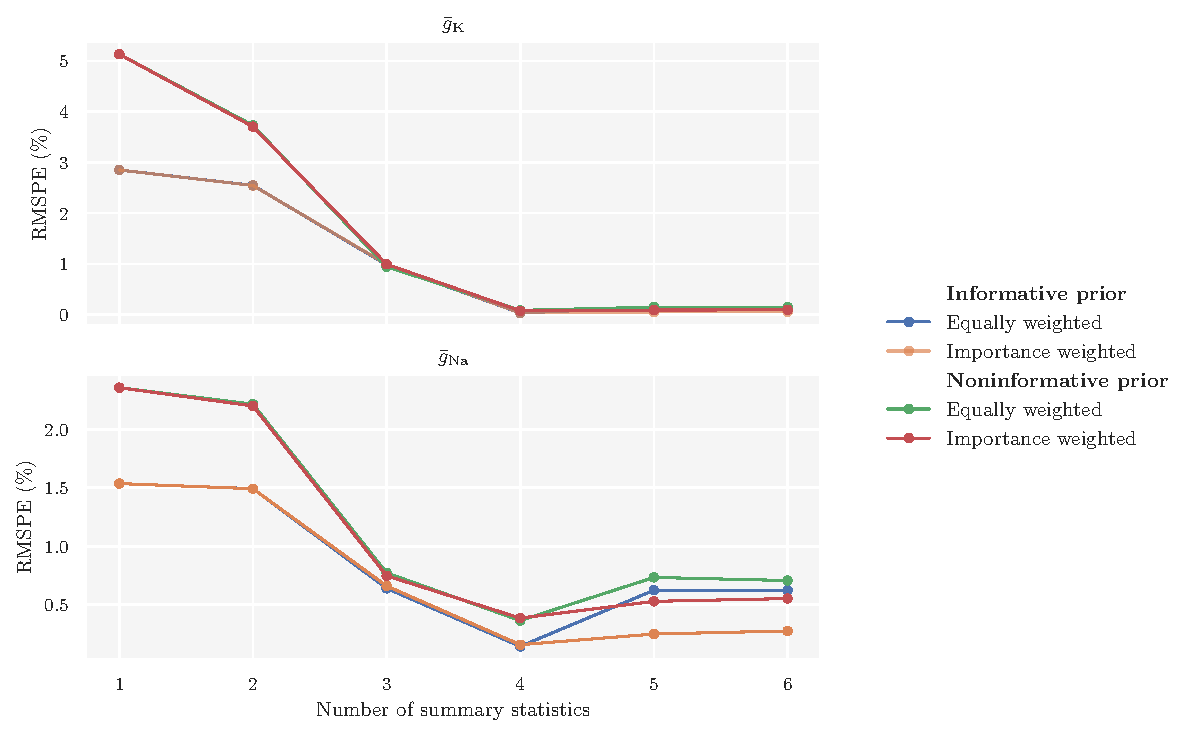
\includegraphics[scale=0.8]{RMSPE_vs_n_sumstats}
    \caption{caption}
    \label{fig:fig1}
\end{figure} 


\subsection{Summarizing Posteriors, informative priors}

Posteriors with original samples, informative prior

\begin{figure}[H]
    \centering
    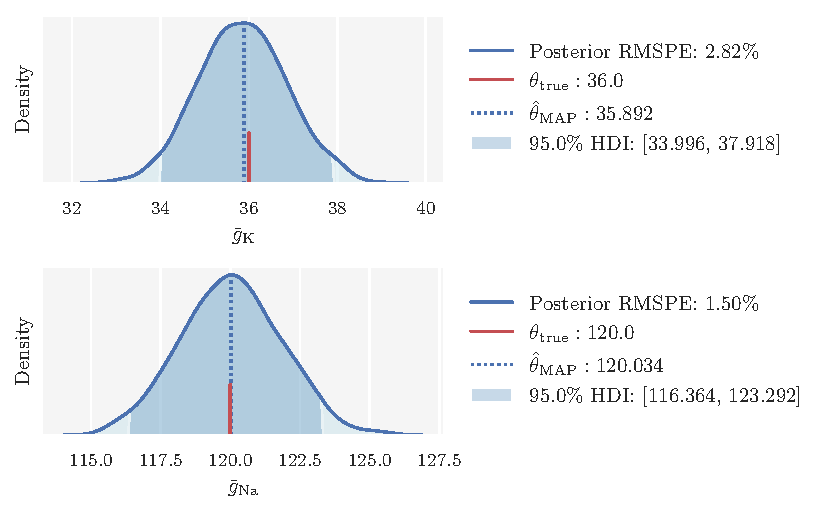
\includegraphics[scale=1]{hh_posterior_org_normal}
    \caption{caption}
    \label{fig:fig1}
\end{figure}

Correlation

\begin{figure}[H]
    \centering
    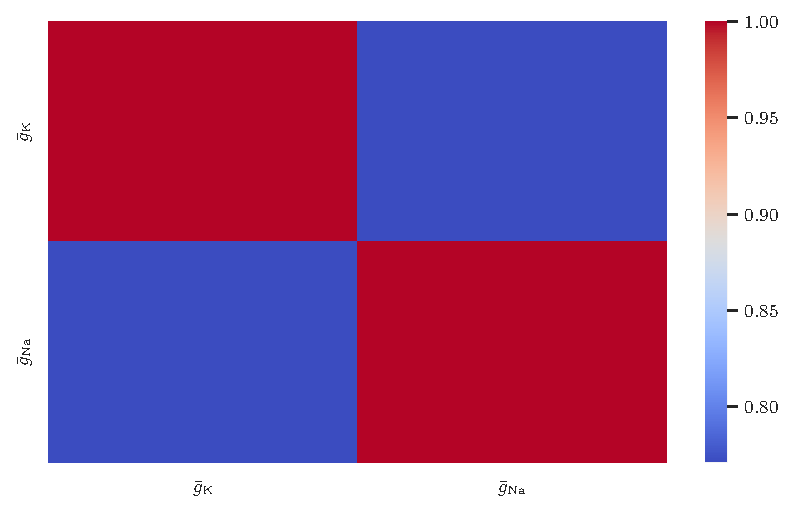
\includegraphics[scale=0.8]{hh_corr_org_normal}
    \caption{caption}
    \label{fig:fig1}
\end{figure}

Joint posterior 

\begin{figure}[H]
    \centering
    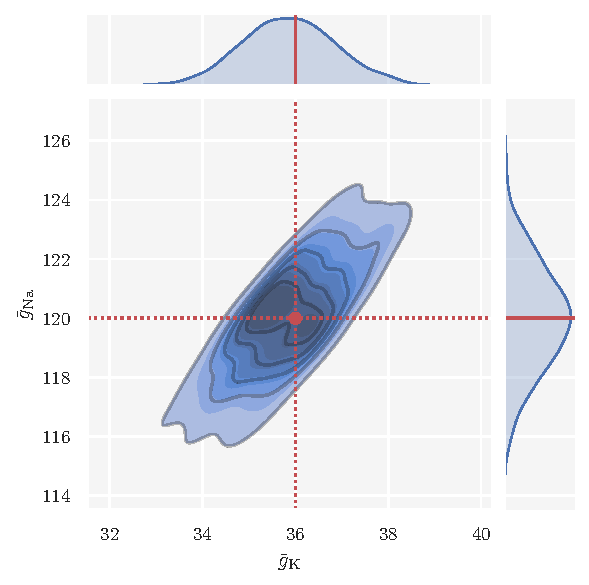
\includegraphics[scale=1.0]{hh_joint_posterior_org_normal}
    \caption{caption}
    \label{fig:fig1}
\end{figure}

Posteriors, reg adjusted samples, informative prior

\begin{figure}[H]
    \centering
    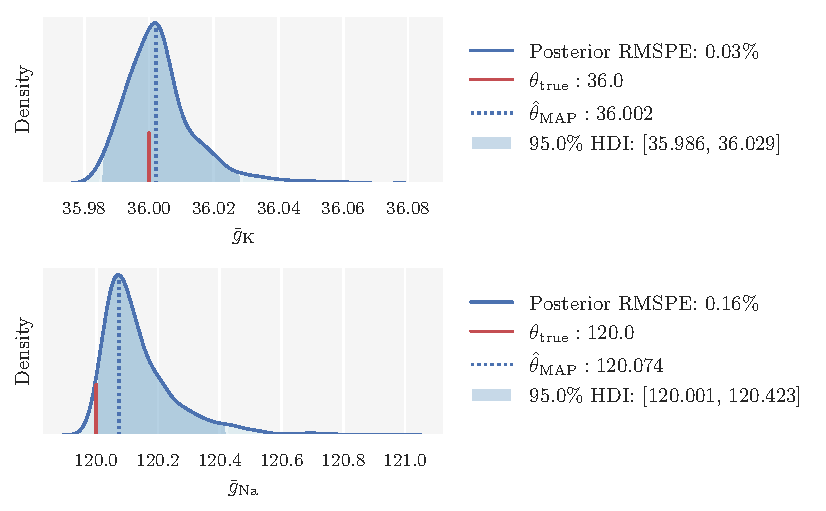
\includegraphics[scale=1.0]{hh_posterior_reg_normal}
    \caption{caption}
    \label{fig:fig1}
\end{figure}

PPC reg adjusted posterior predictive 

\begin{figure}[H]
    \centering
    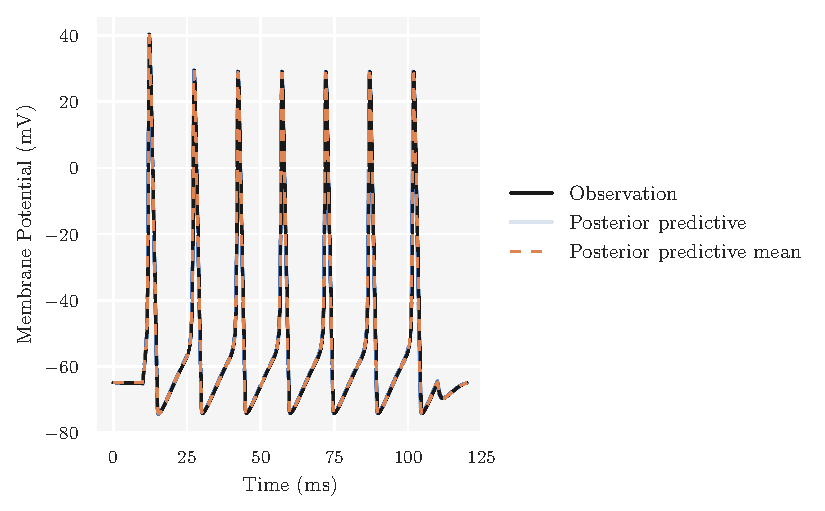
\includegraphics[scale=1.0]{hh_postpred_reg_normal}
    \caption{caption}
    \label{fig:fig1}
\end{figure}


\subsection{Summarizing Posteriors, noninformative priors}

posterior, original, noninfo prior

\begin{figure}[H]
    \centering
    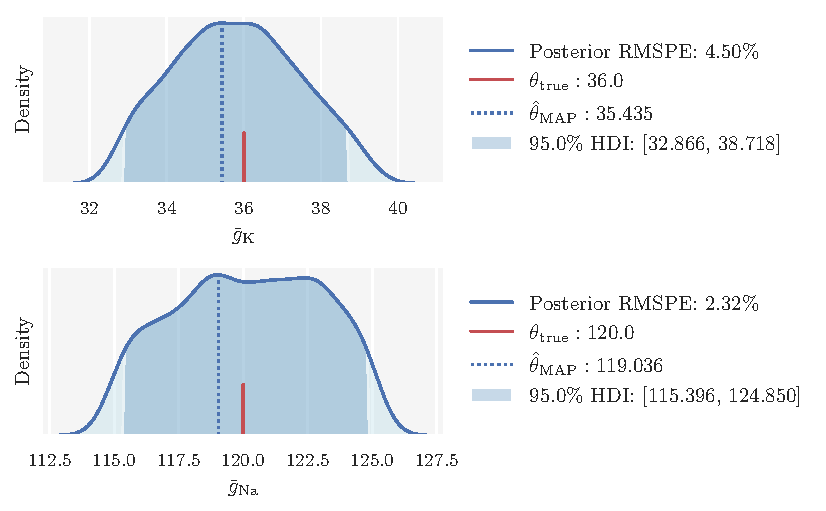
\includegraphics[scale=1.0]{hh_posterior_org_uniform}
    \caption{caption}
    \label{fig:fig1}
\end{figure}

Adjusted posterior, noninformative prior

\begin{figure}[H]
    \centering
    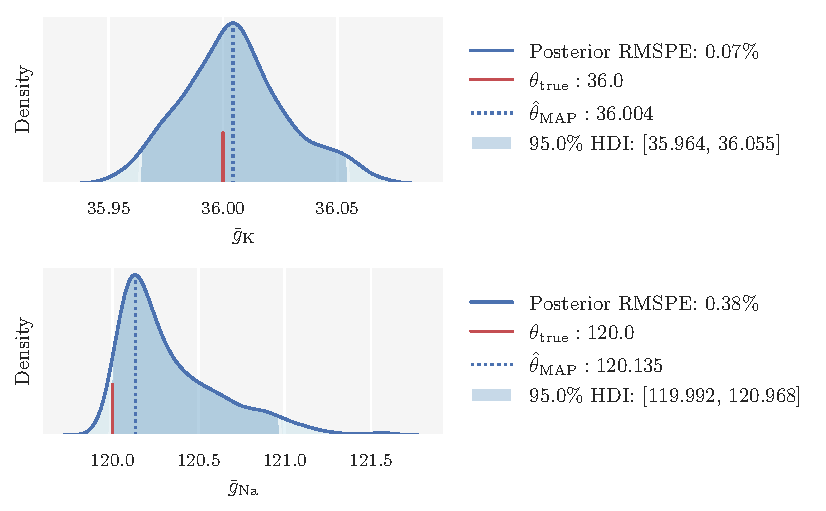
\includegraphics[scale=1.0]{hh_posterior_reg_uniform}
    \caption{caption}
    \label{fig:fig1}
\end{figure} 

PPC adjusted posterior 

\begin{figure}[H]
    \centering
    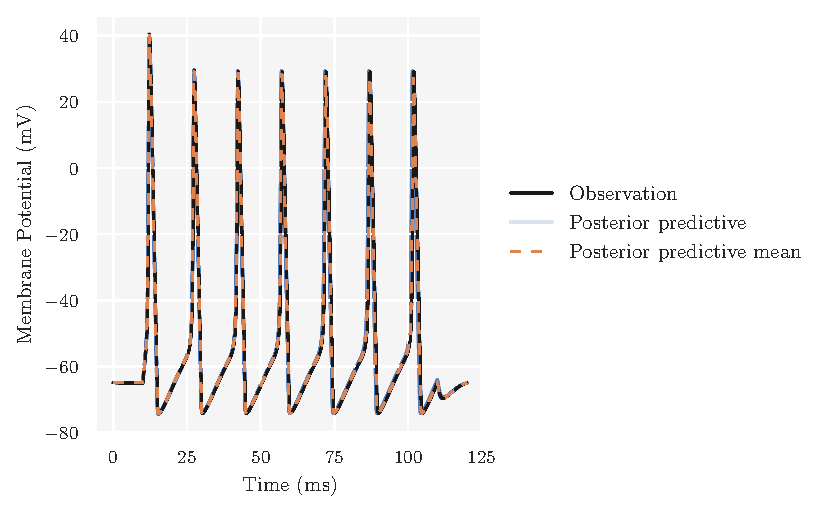
\includegraphics[scale=1.0]{hh_postpred_reg_uniform}
    \caption{caption}
    \label{fig:fig1}
\end{figure}

\subsection{Noisy observation} 

original posterior on noisy observed data

\begin{figure}[H]
    \centering
    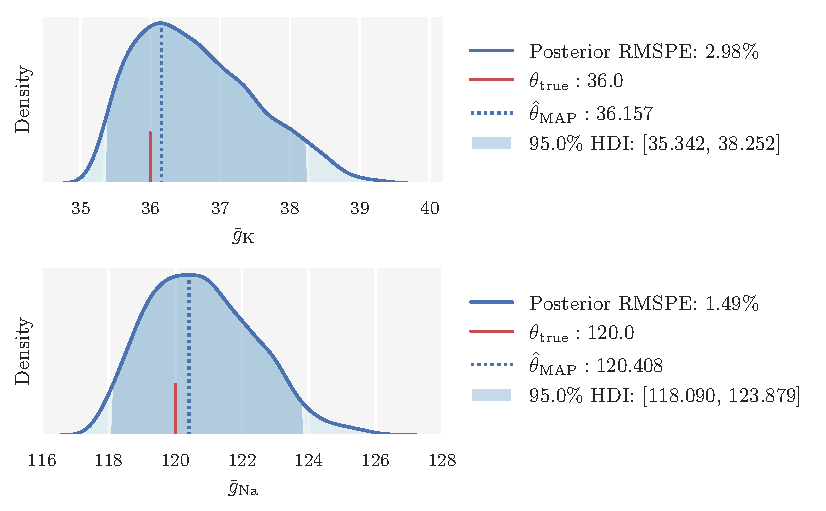
\includegraphics[scale=1.0]{hh_posterior_org_noisy}
    \caption{caption}
    \label{fig:fig1}
\end{figure} 

adjusted posterior on noisy observed data

\begin{figure}[H]
    \centering
    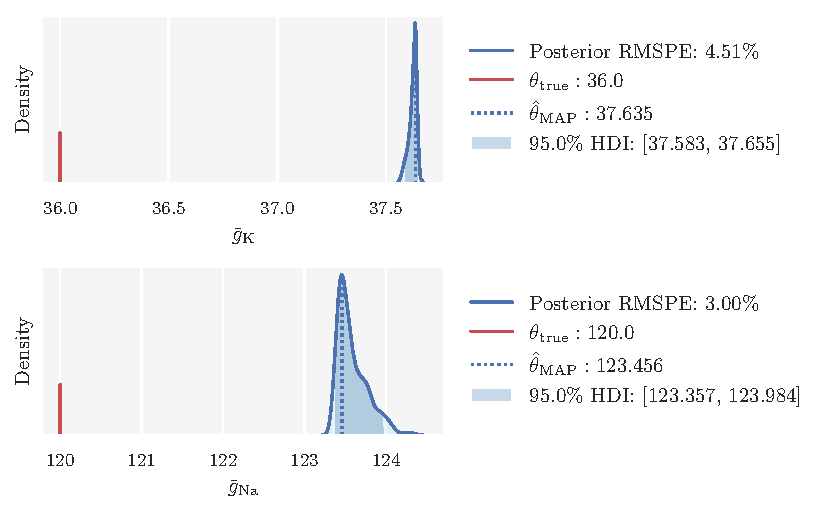
\includegraphics[scale=1.0]{hh_posterior_reg_noisy}
    \caption{caption}
    \label{fig:fig1}
\end{figure} 

ppc with reg adjusted posterior samples (100 posterior samples)


\begin{figure}[H]
    \centering
    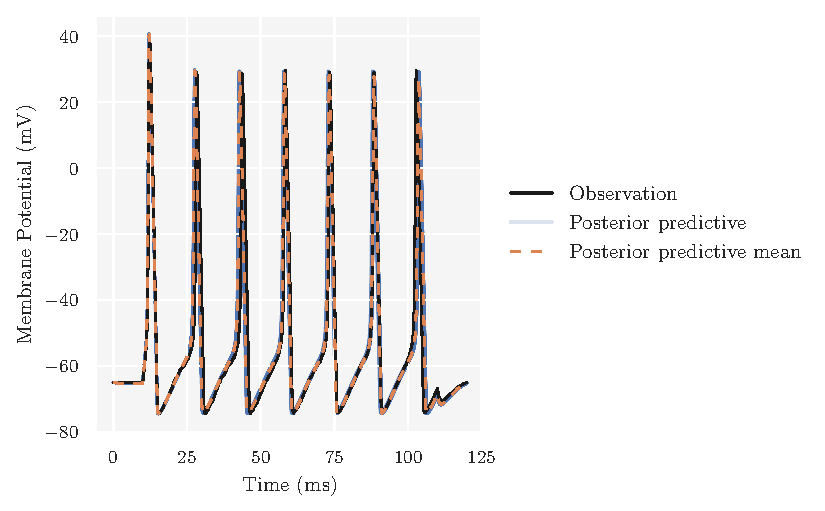
\includegraphics[scale=1.0]{hh_postpred_reg_noisy}
    \caption{caption}
    \label{fig:fig1}
\end{figure}

%================================================================
\section{ABC Settings for Identification of Brunel Network Parameters}
%================================================================

%================================================================
\section{Rejection ABC Posteriors on Synaptic Weight Parameters}
%================================================================

%================================================================
\chapter{Markov Chain Monte Carlo ABC on the Models}
%================================================================